% template from https://tex.stackexchange.com/questions/687422/simple-beamer-template
\documentclass{beamer}
\usecolortheme[named=black]{structure}

\usepackage{graphicx}
\usepackage{url}
\usepackage{minted}
\usepackage{color}

% beamer theming
\usefonttheme[onlymath]{serif}
\setbeamertemplate{frametitle}[default][center]
\setbeamerfont{frametitle}{series=\bfseries}

\title{Formal Methods}
\author{M. Nimalan}
\date{\today}

\setbeamertemplate{navigation symbols}{}
\setbeamertemplate{page number in head/foot}[totalframenumber]
\setbeamertemplate{footline}[text line]{\insertshorttitle\hfill\usebeamertemplate{page number in head/foot}}

% from https://tex.stackexchange.com/a/329929/36296
\makeatletter
\setbeamertemplate{theorem begin}{%
%  \begin{\inserttheoremblockenv}% removed
  {%
    {\bfseries\inserttheoremname
    \ifx\inserttheoremaddition\@empty\else\ (\inserttheoremaddition)\fi}%
    \space% new
  }%
}
\setbeamertemplate{theorem end}{}
\makeatother
\setbeamertemplate{itemize item}[circle]


\begin{document}

\frame{\titlepage}

\begin{frame}{Let's start with some questions}
  \begin{columns}
    \begin{column}{0.5\textwidth}
      \begin{itemize}
        \item Given integers $x$ and $y$ can the this equation be solved?
        \item How did we know that this does not have a solution?
        \item Can we generalize the way we solve this?
        \item Given any set of equations is there a way to know if the exists a solution that \textbf{satisfies} the equations
      \end{itemize}
    \end{column}

    \begin{column}{0.5\textwidth}
      $$ x + y = 5 $$
      $$ 2x + 2y = 15$$
    \end{column}
  \end{columns}
\end{frame}

\begin{frame}{Valid and Satisfiable}
  \begin{itemize}
    \item \textbf{Valid} An set of equations are valid if they are true for all assignment of values to its variables.
    \item \textbf{Satisfiable} An set of equations are satisfiable if it is true for some assignment of values to its variables.
    \item ...
    \item We can prove a set of equations to be \textbf{Invalid}, by proving that the opposite is \textbf{Satisfiable}
  \end{itemize}
\end{frame}

\begin{frame}[fragile]{Satisfiability Modulo Theory}
  \begin{columns}
    \begin{column}{0.5\textwidth}
      Formal Solvers
      \begin{itemize}
        \item Satisfiability Modulo Theory is the problem of determining whether a 
      mathematical formula is satisfiable.
        \item Theorm Provers are tools that test whether given model is satisfiable eg) z3
        \item Models are written SMT Lib, and a Theorm Provers solves these models.
      \end{itemize}
    \end{column}
    \begin{column}{0.5\textwidth}
      \begin{center}
        \textbf{SMT Lib}
      \end{center}
      \begin{minted}{cl}
(declare-const x Int)
(declare-const y Int)

(assert (= (+ x y) 5))
(assert (= (+ (* 2 x) (* 2 y)) 15))

(check-sat)
      \end{minted}
    \end{column}
  \end{columns}
\end{frame}

\begin{frame}{SAT and SMT}
  \begin{itemize}
    \item Boolean Satisfiability problem (SAT) solvers find variable assignments that solve boolean formula
    \item Satisfiability Modulo Theory (SMT) solvers has theories beyond boolean formulas
  \end{itemize}
\end{frame}

\begin{frame}{Application of Formal Methods}
  If you want to prove a design/algorithm/model correct, you model it in SMT lib and use a theorm solver to prove it.

  \begin{itemize}
    \item Formal Verification of hardware
    \item Contraint problems
    \item Security Research
    \item Design of Cryptographic Algorithms
  \end{itemize}
\end{frame}

\begin{frame}{Formal Verification of Hardware}
  \begin{figure}[h]
    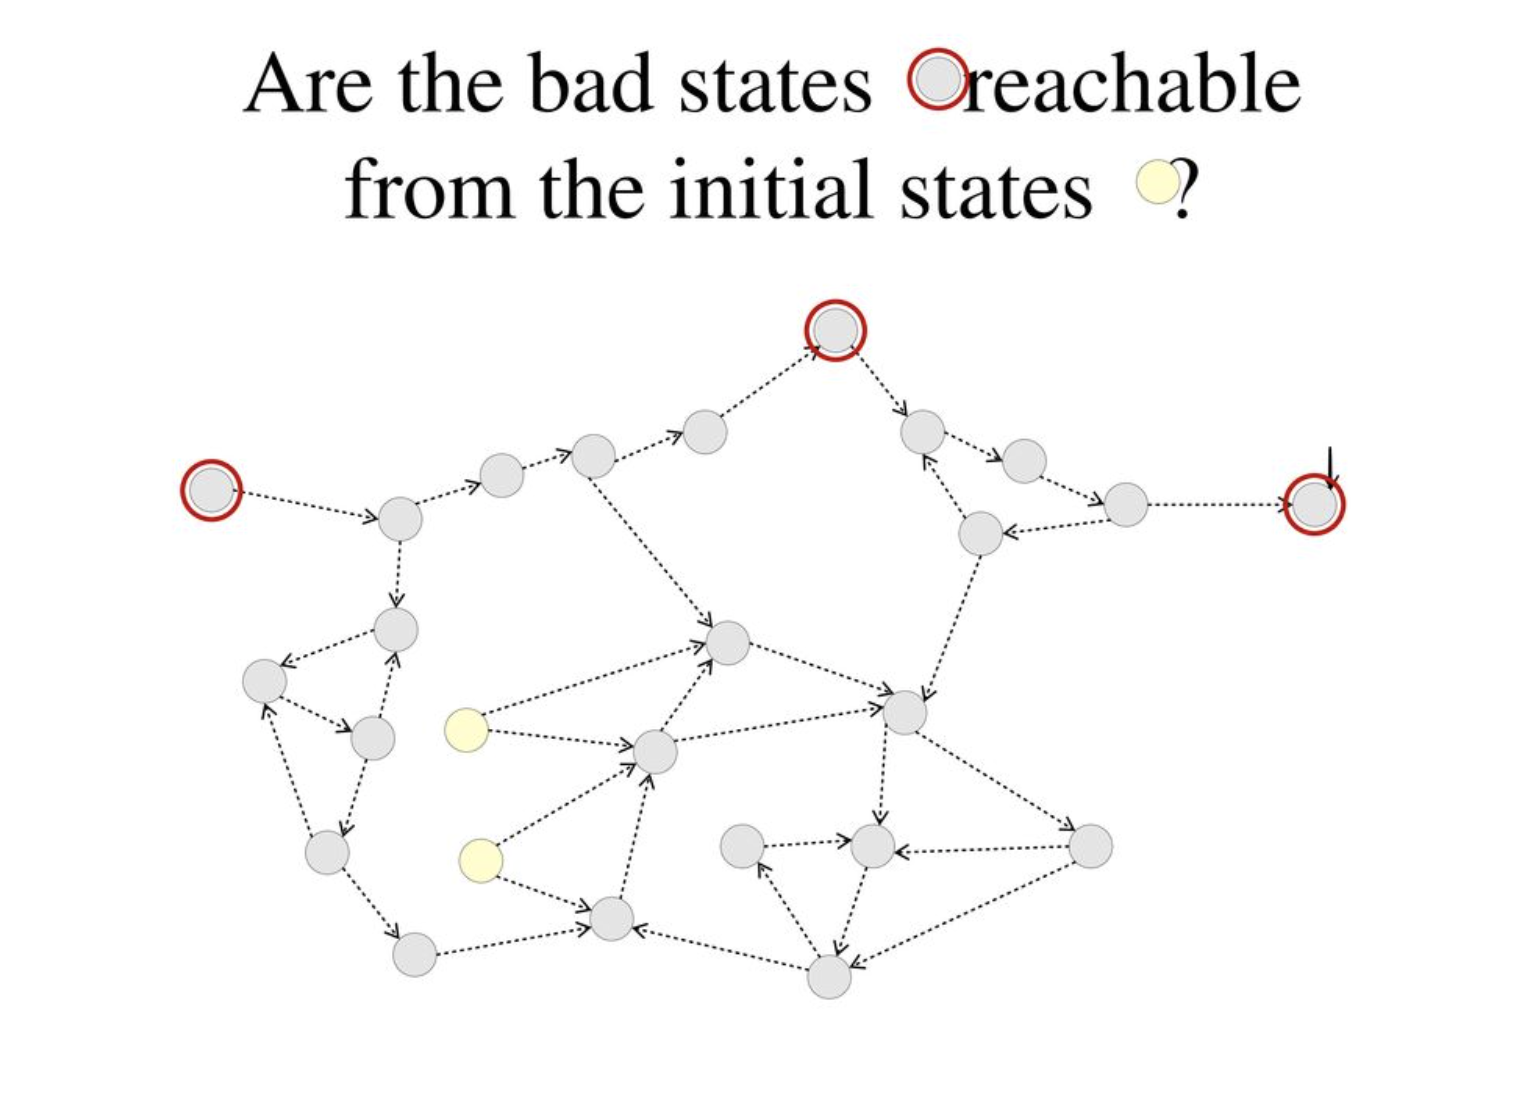
\includegraphics[width=\textwidth]{formal_1}
    \scriptsize Image Credit: Clifford Wolf, Formal Verification with SymbiYosys and Yosys-SMTBMC
  \end{figure}
\end{frame}

\begin{frame}{Formal Verification of Hardware}
  \begin{figure}[h]
    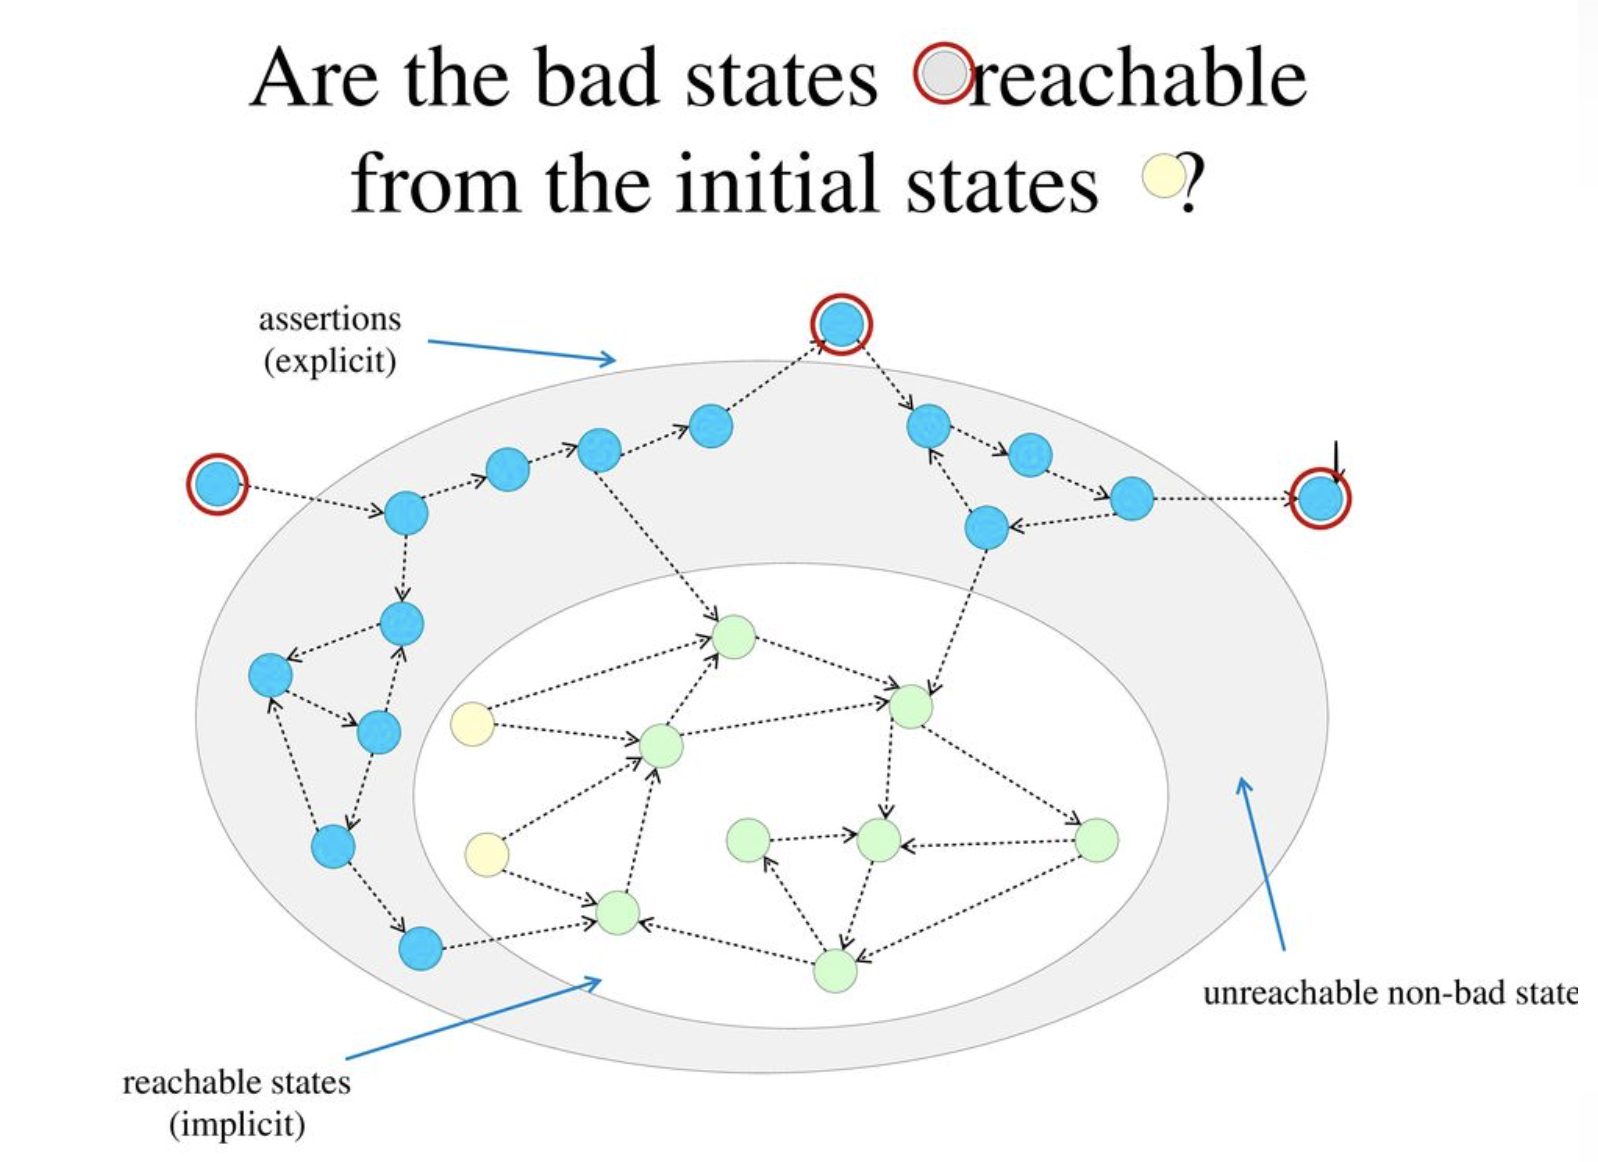
\includegraphics[width=\textwidth]{formal_2}
    \scriptsize Image Credit: Clifford Wolf, Formal Verification with SymbiYosys and Yosys-SMTBMC
  \end{figure}
\end{frame}

\begin{frame}
  \begin{figure}[h]
    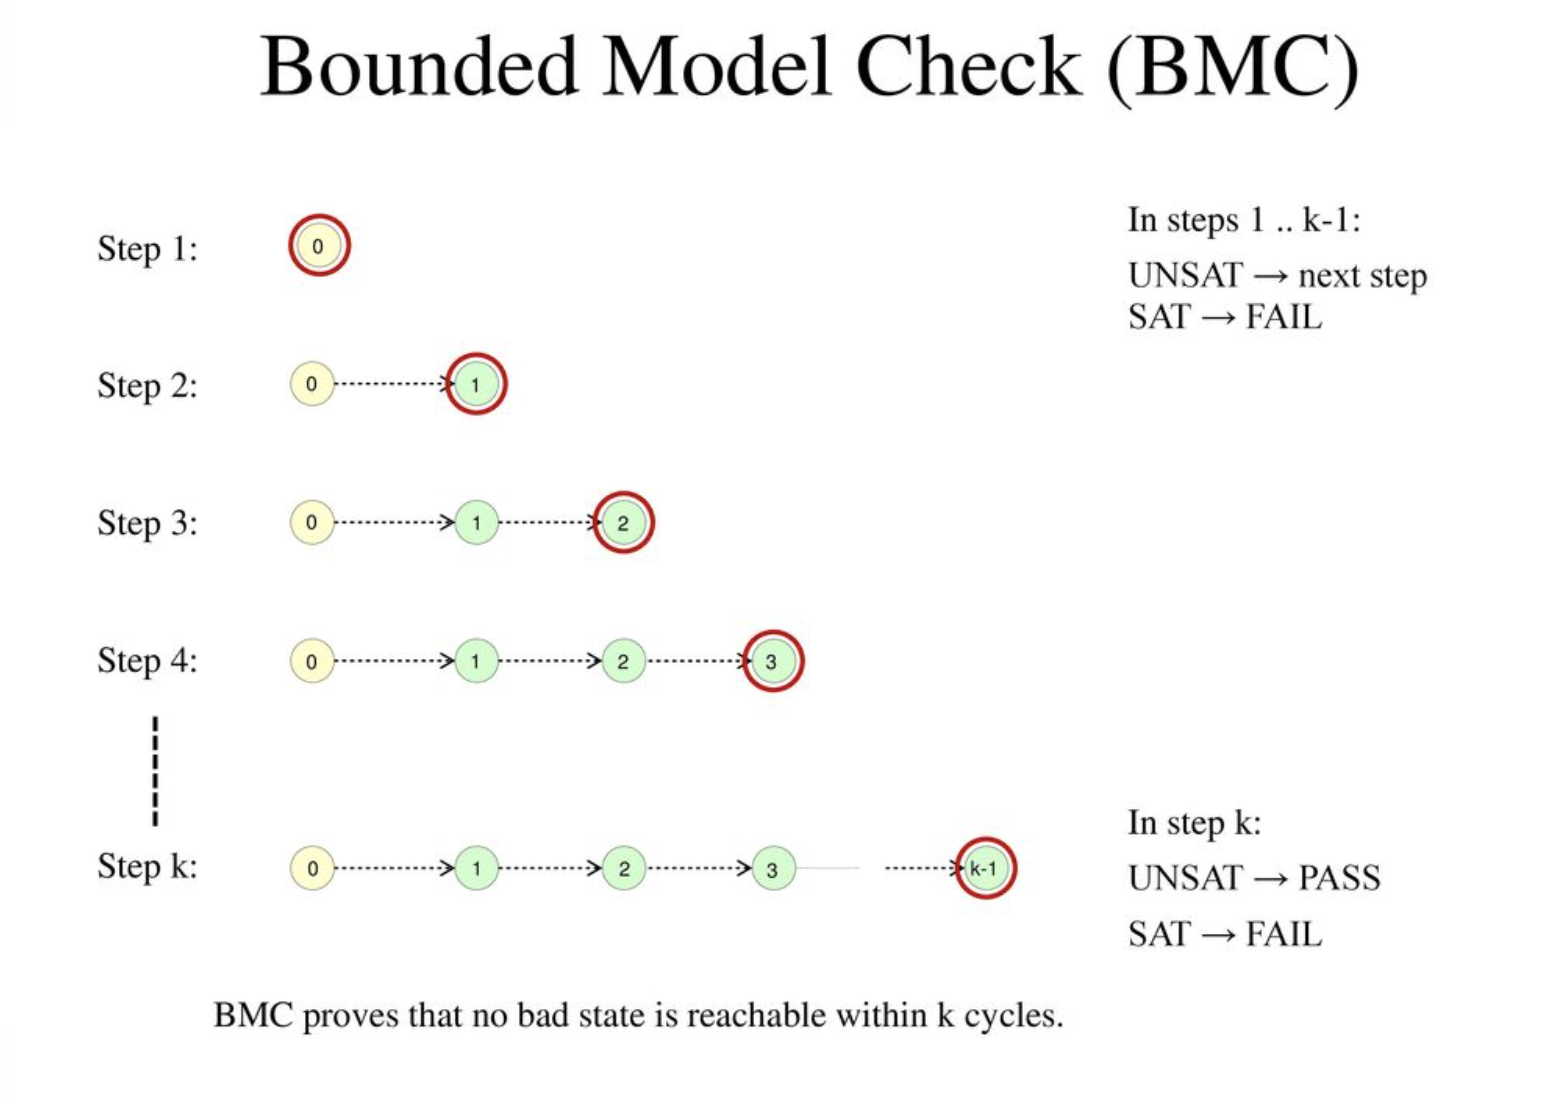
\includegraphics[width=\textwidth]{formal_3}
    \scriptsize Image Credit: Clifford Wolf, Formal Verification with SymbiYosys and Yosys-SMTBMC
  \end{figure}
\end{frame}

\begin{frame}
  \begin{figure}[h]
    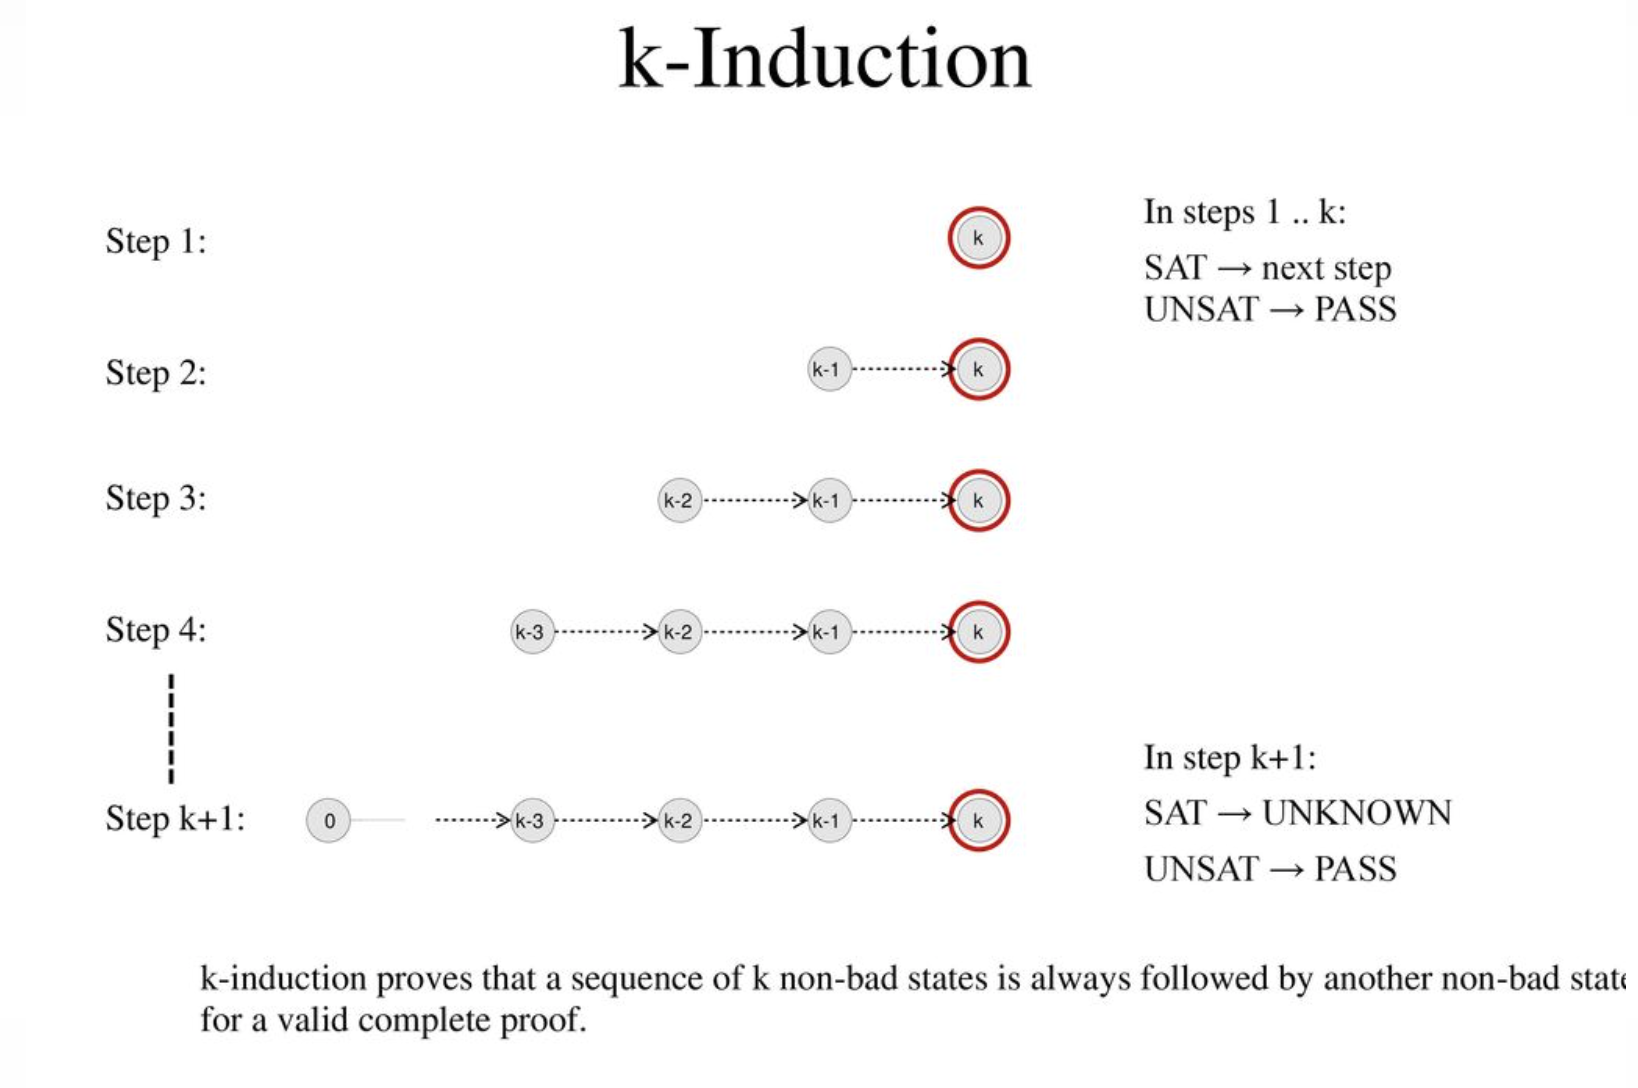
\includegraphics[width=\textwidth]{formal_4}
    \scriptsize Image Credit: Clifford Wolf, Formal Verification with SymbiYosys and Yosys-SMTBMC
  \end{figure}
\end{frame}

\begin{frame}{Reading}
  \tiny
  \begin{itemize}
    \item \url{https://theory.stanford.edu/~nikolaj/programmingz3.html}
    \item \url{https://slideplayer.com/slide/11950984/}
    \item \url{https://link.springer.com/chapter/10.1007/978-3-642-22110-1_46}
    \item \url{https://www.microsoft.com/en-us/research/wp-content/uploads/2013/07/SMT13.pdf}
    \item \url{https://davidsherenowitsa.party/2018/09/19/solving-logic-puzzles-with-z3.html}
    \item \url{https://stackoverflow.com/questions/14547087/extracting-bits-with-a-single-multiplication/14551792}
  \end{itemize}
\end{frame}

\begin{frame}{Thank You}
  \begin{center}
    A presentation by M.Nimalan (@mark1626)
    \begin{figure}[h]
      
\includegraphics{cc_by}
    \end{figure}
  \end{center}
\end{frame}

\end{document}
